%%%% 第一版 2020.10
%此文档为普通物理实验三林伟华老师要求的物理实验报告模板
%作者:武汉大学物理科学与技术学院18级詹睿知
%参考自电子信息学院实验报告模板
%%%% 第二版 2022.8
%更改优化了documentclass
\documentclass{WHUReport}
\usepackage[]{amsmath}
\usepackage{natbib}
\setcitestyle{numbers,square}
\usepackage{amsmath}
\usepackage{esint}

%%%% 以下填写学生信息及实验题目
\newcommand{\major}{物理学}
\newcommand{\name}{郑卜凡}
\newcommand{\stuid}{2021302022016}
\newcommand{\Name}{Bufan Zheng}
\newcommand{\course}{普通物理实验三}
\newcommand{\newtitle}{数字全息干涉记录与再现}
\newcommand{\Title}{Digital Holographic Interference Recording and Reproduction}

\begin{document}
\pagestyle{maincontent} 
%\bibliographystyle{plain}

\begin{center}
\zihao{-2} \textbf{\newtitle}\\
\zihao{7}~\\
\zihao{4} \kaishu \name \ \ (\stuid)\\
\zihao{5} \kaishu (武汉大学物理科学与技术学院,湖北省 武汉市 430072)\\
\end{center}
\zihao{-5}\textbf{摘\quad 要:}
%在此处修改中文摘要
本实验搭建全息干涉光路并数字采集全息图,然后通过软件再现物信息,实现光学记录和数字再现。并利用计算机模拟计算全息图,与采集图样进行比对分析。还利用模拟计算得到的全息图通过空间光调制器光学再现出了原物图像。\\
\zihao{-5}\textbf{关键词:}全息干涉,数字全息,计算模拟全息,光学实时再现。
~\\
\begin{center}
	\zihao{3}\textbf{\Title}\\
	\zihao{-4} \Name\quad (\stuid)\\
	\zihao{5} School of physical science and technology, Wuhan University, Wuhan, 430072, China
\end{center}

\zihao{5}\textbf{Abstract:}This experiment builds a holographic interference optical path and digitally collects holograms, and then reproduces the object information through software to achieve optical recording and digital reproduction. The holograms were simulated and calculated using a computer, and compared and analysed with the collected samples. The simulated holograms were also used to optically reproduce the original image of the object through a spatial light modulator.\\
\zihao{5}\textbf{Keywords: }Holographic interference, digital holography, computational analogue holography, optical real-time reproduction.

\begin{multicols}{2}
	光是一种电磁波,不仅具有振幅,还具有相位,但是传统光学测量都只能得到振幅信息,相位信息完全丢失,这使得我们不可能从一幅照片中还原得到真实物体的全部信息。全息技术是基于光的干涉原理,将物体发射光波波前以干涉的形式记录光波的相位和振幅信息,利用光的衍射理论再现所记录物光波的波前,从而获得物体振幅和相位信息。普通光学全息技术是利用高分辨率的记录介质,如银盐干版,来记录干涉图,经过化学处理后形成全息图,在照明光照射下再现出原物体的三维形貌 (包括振幅和相位)的一种技术.光学全息干版需要经过暗房处理,难以实现实时数字化处理,也对被记录信息的保存、传送带来不便。
	
	1967年Goodman提出数字全息\upcite{ref1},它是一种光电混合系统,其记录光路和普通全息基本相同,不同的是用摄像机等光敏器件代替普通的全息干版来拍摄全息图, 并将记录的全息图采集到计算机, 然后用数值计算的方法对全息图进行再现。它相比于传统的光学全息来说具有很大优点和灵活性,它摆脱了传统的化学湿处理,可以实现物光场的实时再现。同时,利用数字全息独特的数值再现技术,可以分别获得定量的光波场振幅和相位信息。可惜的是,由于数字全息对记录设备的分辨率和计算机的性能要求较高, 此方法在提出后很长一段时间进展缓慢。进入21世纪,高性能计算机和高分辨CCD电荷耦合器件飞速发展,数字全息已应用于三维相衬成像、微结构检测等许多领域\upcite{ref2,ref3,ref4,ref5},是当前光学检测和信息处理的研究前沿。
	
	本文将简要介绍全息技术的原理,并利用实验直观的展示了数字全息这一新兴活跃的光学领域的不同方面\upcite{ref6}。有便于更好的理解背后的光学原理。
	\section{数字全息的记录和再现原理}
	\subsection{数字全息的记录}
	为了解决直接在探测平面上探测丢失相位分布的问题,可以引入一束复振幅分布已知的光波(本实验使用氦氖激光器产生),称为参考光波与物质光波干涉并记录其干涉图样,也就是所谓的数字全息图。然后利用计算机反向解算出物光波在探测平面上的复振幅,反向传播到物平面就可以重建出清晰的图像了。
	
	假设物平面为$x_0\mbox{-}y_0$,记录平面为$x\mbox{-}y$,物光场分布为$U_0(x_0,y_0)$,可以利用菲涅尔公式计算其传播到记录平面上的光场分布:
	\begin{equation}
		\begin{aligned}
			O(x,y)=& \frac{1}{\operatorname{i}\lambda {z}}\mathrm{e}^{\operatorname{i}\frac{2\pi}{\lambda z}}\mathrm{e}^{\operatorname{i}\pi\frac{(x^2+y^2)}{\lambda  z}}\cdot\\
			&\iint U_0(x_0,y_0)\mathrm{e}^{\mathrm{i}\pi{\frac{x_0^2+y_0^2}{\lambda  z}}}\mathrm{e}^{-\mathrm{i}2\pi\frac{x_0x+y_0y}{\lambda z}}\mathrm{d}x_0\mathrm{d}y_0\\
			\equiv&A_{0}(x,y)\exp[\mathrm{i}\varphi_{0}(x,y)]
		\end{aligned}
	\end{equation}
	记录平面上的参考光波记为:
	\begin{equation}
		R(x,y)=A_{r}(x,y)\exp[\mathrm{i}\varphi_{r}(x,y)]
	\end{equation}
	其中$A_r$和$\varphi_r$是已知的。则全息图上光场强度分布为:
	\begin{equation}
		\begin{aligned}I_{\mathrm{H}}(x,y)=&\left|A_{\mathrm{O}}(x,y)\right|^2+\left|A_{\mathrm{r}}(x,y)\right|^2+O(x,y)R^{^*}(x,y)\\&+O^{^*}(x,y)R(x,y)\\=&\left|A_{\mathrm{O}}(x,y)\right|^2+\left|A_{\mathrm{r}}(x,y)\right|^2\\&+2A_{\mathrm{O}}(x,y)A_{\mathrm{r}}(x,y)\cos[\varphi_{\mathrm{O}}(x,y)-\varphi_{\mathrm{r}}(x,y)]\end{aligned}
	\end{equation}
	而强度分布是很好测量的,我们成功的利用干涉将相位信息转化为了强度信息记录下来!CCD记录全息图是离散的数字采样,可以用下面的公式表示:
	\begin{equation}
		\begin{aligned}
			I(u,v)=&I_{\mathrm{H}}(x,y)\operatorname{rect}(\frac{x}{L_x},\frac{y}{L_y})\cdot\\&\sum_{u=-\frac{N_x}2}^{\frac{N_x}2-1}\sum_{\nu=-\frac{N_y}2}^{\frac{N_y}2-1}\delta(x-u\Delta x,y-\nu\Delta y)
		\end{aligned}
	\end{equation}
	这里$N_x\times N_y$表示离散化后的数字点阵大小,$L_x\times L_y$表示CCD的光敏面尺寸,$\Delta x\equiv L_x/N_x,\Delta y\equiv L_y/N_y$表示采样间隔。
	
	根据奈奎斯采样定理\upcite{ref7},只有当记录介质的空间频率是全息图表面上光波的空间频率的两倍以上时,才能重现出高分辨率的原物图像。由于摄像机分辨率(约100线/mm)比全息于板等传统记录介质的分辨(约5000线/mm)低的多,而且CCD靶面较小,这一条件很难被满足,所以必须合理设计光路以重现出清晰的像。利用采样定理,可以做如下计算,设物光和参考光在全息图表面上的最大夹角为$\theta_\mathrm{nax}$,则摄像机平面上形成最小的条纹间距$\Delta e_\mathrm{min}$为:
	\begin{equation}
		\Delta e_{\min}=\frac{\lambda}{2\sin(\theta_{\max}/2)}
	\end{equation}
	由于$e_{\min}\geq 2\Delta x$,所以最终参考光和物光之间的最大夹角应该满足:
	\begin{equation}
		\theta_{\max}\leq\frac\lambda{2\Delta x}
	\end{equation}
	摄像机尺寸取为$5\operatorname*{\mu m}$,$\lambda$取为绿光$532\operatorname*{nm}$,得到$\theta_{\max}\approx 3.04^\circ$。所以后面在调节光路的时候,干涉条纹会尽量调的密一些(大致和指纹的间距相同),这样才能保证最后重现出来的图像分辨率更高。
	\subsection{数字全息的再现}
	假设物体平面到记录平面的距离为$z$,由于参考光已知,所以利用全息图首先可以计算得到物质光波场在记录平面的复振幅,然后只需要利用菲涅尔衍射过程反向传播$z$距离就可以得到物质光波波场,假设数字再现平面为$x_I\mbox{-}xy_I$,有公式:
	\begin{equation}\label{eq}
		\begin{aligned}
			U_{\mathrm{I}}(x_{\mathrm{I}},y_{\mathrm{I}})=&\frac{\exp(\mathrm{i}kz)}{\mathrm{i}\lambda z }\int_{-\infty}^{\infty}\int_{-\infty}^{\infty}I(u,v)C(u,v)\times\\&\exp\{\frac{\mathrm{i}k}{2d}[(x_{\mathrm{I}}-u)^{2}+(y_{\mathrm{I}}-v)^{2}]\}\mathrm{d}u\mathrm{d}v\\
			\approx& \frac{\exp(\mathrm{i}kz)}{\mathrm{i}\lambda z}\exp[\frac{\mathrm{i}k}{2z}({x_{\mathrm{I}}}^{2}+{y_{\mathrm{I}}}^{2})]\times   \\
			&\int_{-\infty}^{\infty}\int_{-\infty}^{\infty}I(u,v)C(u,v)\exp[\frac{\mathrm{i}k}{2z}(u^{2}+v^{2})]\\&\exp[-\frac{\mathrm{i}2\pi}{\lambda z}(ux_{I}+\nu y_{I})]\operatorname{d}u\operatorname{d}v
		\end{aligned}
	\end{equation}
	为了成像清晰再现距离$|z|$必须等于记录距离$d$,如果是正向传播$z=d$,则再现像是=物光波共轭像;如果是反向传播$z=-d$,则再现像包含物光波的所有振幅相位信息。无论什么衍射距离的选取,都可以利用公式\ref{eq}进行数值计算。
	
	数字像面全息图是物光场的像与参考光在全息平面干涉的强度分布$I_{\mathrm{H}}(x,y)$。因此$I(\mu,\nu)$ 的傅里叶变换频谱$I(f_a,f_v)$将包含原始物光波的频谱,同时存在物光共轭像的频谱及零级衍射光。如果利用频谱滤波技术\upcite{ref9}或在参考光中引入相移\upcite{ref8}等方法消除共轭像的频谱及零级衍射光,这样就将得到物光场在全息平面$x\mbox{-}y$面上的像的频谱$I_{\mathrm{o}}(f_u,f_v)$, 再通过傅里叶反变换,就可以获得物光场的像的复振幅分布$U_1(x_1,y_1)$。
	\section{光学再现}	
	前面数字再现本质上就是去用计算机模拟光波衍射,这当然也可以直接,通过搭建光路衍射实现。当然,光线不能反向传播,所以我们只能得到物质光场的共轭场,但是这只需要再加一个凸透镜,在一倍焦距到两倍焦距之间合适位置放摄像机,即可得到物质光场共轭场的共轭场,也就是物质光场本身。还有一个要点是要将记录的全息图加载到光路之中,这可以使用空间光调制器实现。空间光调制器可以粗浅的理解为一个分辨率很高的显示屏,可以自动的对加载到上面的全息图进行相位调制和振幅调制,就可以加载到光路中使用进行再现了。这一点更加详细的介绍可见文献\cite{ref10}。
	\section{计算模拟全息}
	一旦物质本身已知,那么它的光场也是已知的,所以我们完全可以使用计算机去计算最终得到的全息图,这和搭建光路去记录全息图是完全等价的。而且由于计算机计算没有考虑实验误差和各种环境干扰,得到的全息图像更加精确\upcite{ref11}。
	
	对于傅里叶变换全息图,全息图上记录的是物波的空间频谱,而且数字记录得到的是离散采样,所以必须进行离散傅里叶变换:
	\begin{equation}
		F(j,k)=\sum_{m=-\frac M2}^{\frac M2-1}\sum_{m=-\frac N2}^{\frac N2-1}f(m,n)\exp[-\mathrm{i~}2\pi(\frac{jm}M+\frac{kn}n)]
	\end{equation}
	快速傅里叶变换(FFT)算法的发明极大的减少了这一计算所需的时间,促进了计算全息领域的发展。Lohmann等人提出了迂回相位型计算全息图的编码方法将计算出的全息图面上的复振幅函数转化成实值函数编码成灰度图。这一问题牵扯到的理论十分复杂,详见文献\cite{ref12}。
	\section{透射数字全息实验}
	根据前面的分析,首先需要搭建干涉光路(马赫曾德干涉光路)在摄像机平面内获得全息图并拍摄:
	\begin{figure}[H]
		\centering
		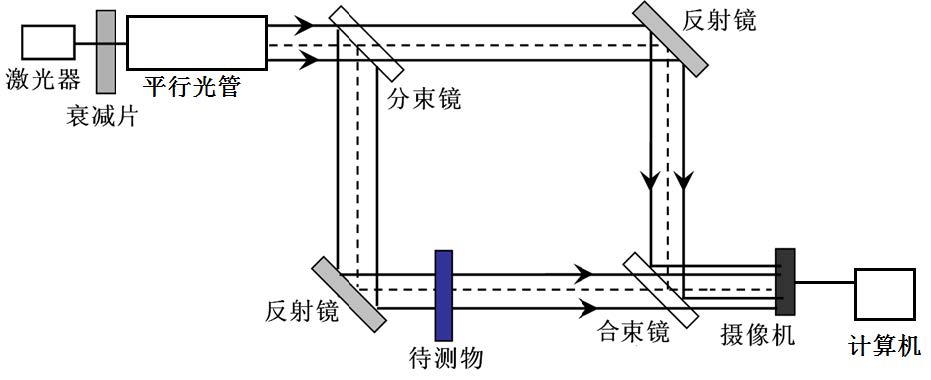
\includegraphics[width=\linewidth]{figs/透射全息.jpg}
		\caption{马赫曾德干涉光路}
	\end{figure}
	如果调节好了光路平行,移动平行光管应当观测到光斑大小不变。另外非常重要的一点是要调节分束镜的角度使得条纹间距与指纹差不多,前面分析过这是为了满足采样定理。摄像机与待测物的距离可用公式 $\Delta L_0=\lambda d/p$ 确定,式中 $\Delta L_{\mathrm{o}}$为物体尺寸的 4倍,$\lambda$ 是光波长,$d$ 为记录距离,$p$ 为 CCD 的像元尺寸。实验中物体尺寸为$20\operatorname{mm}\times 20\operatorname{mm}$, CCD 像素为 5.2μm, 光波长是 532nm, 所以记录距离可选择 150mm\mbox{-}450mm。
	
	对两个物体分别进行拍摄,得到全息图:
	\begin{figure}[H]
		\centering
		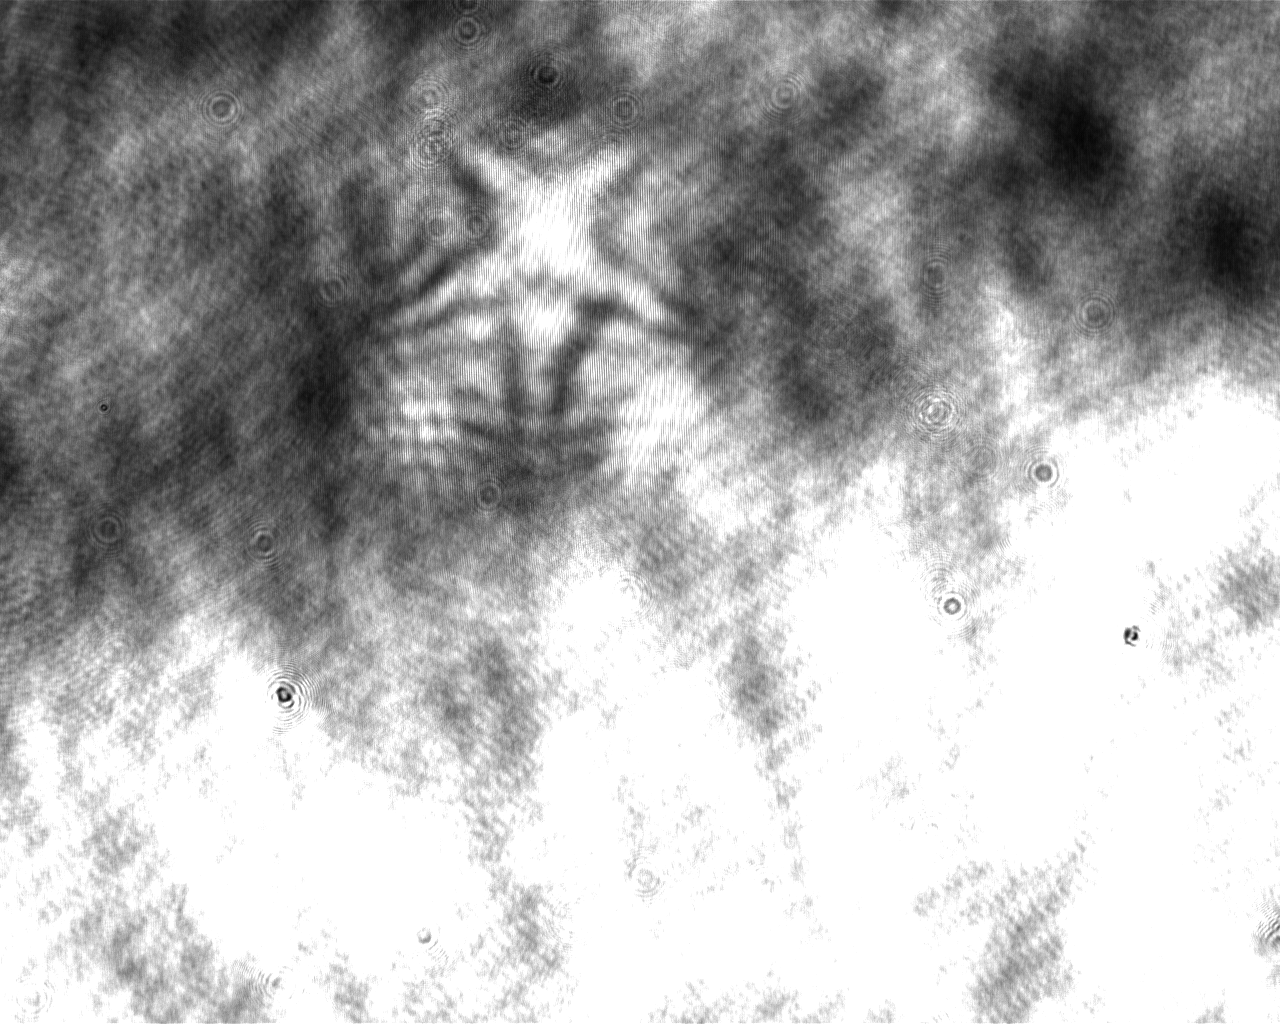
\includegraphics[width=.8\linewidth]{figs/1.png}
		\caption{全息图一}
		\label{fig1}
	\end{figure}
	\begin{figure}[H]
		\centering
		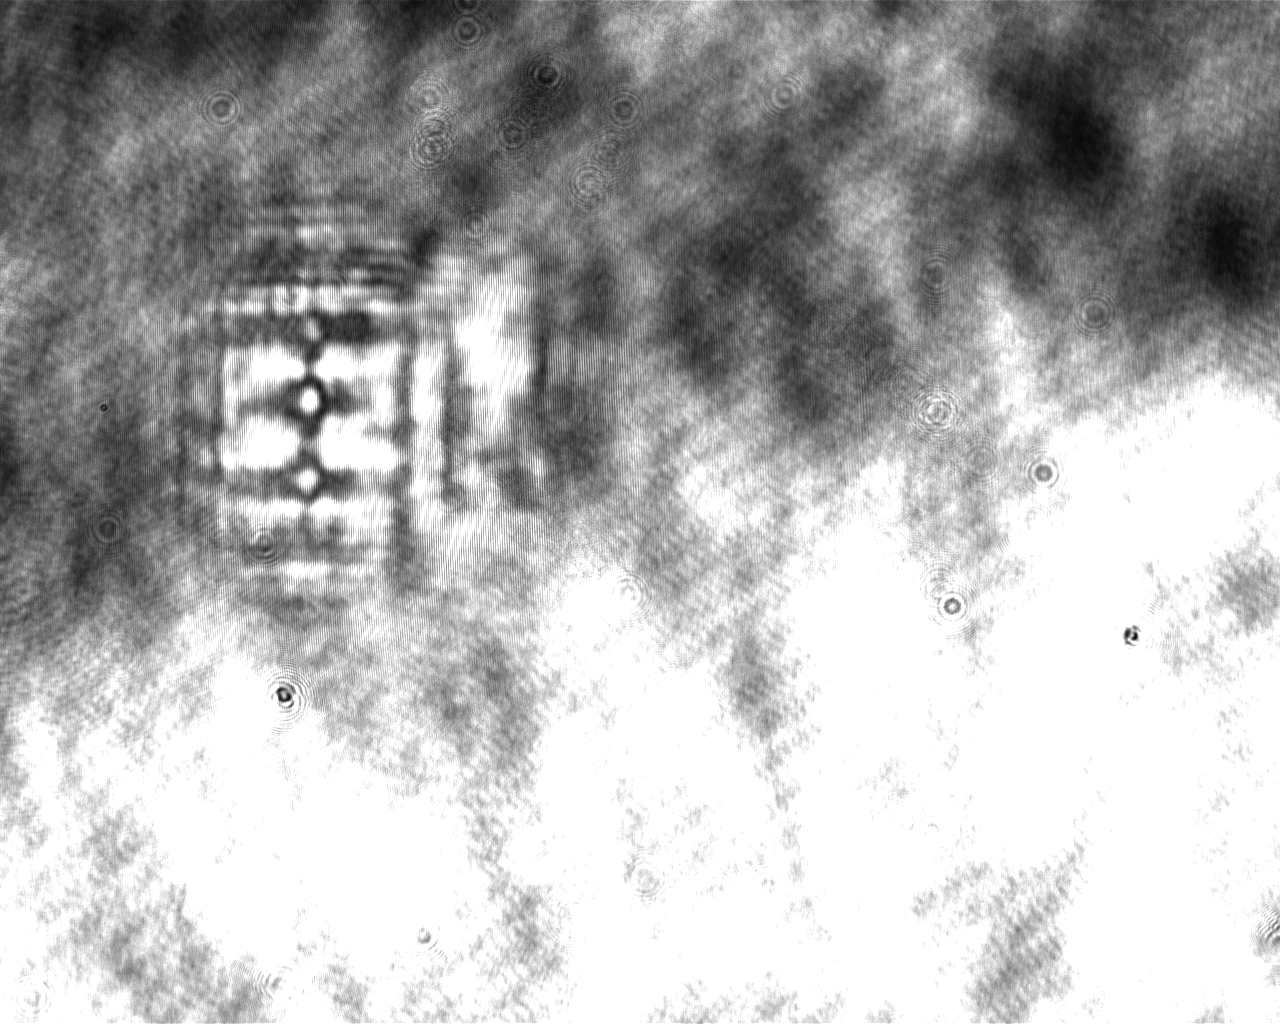
\includegraphics[width=.8\linewidth]{figs/2.png}
		\caption{全息图二}
		\label{fig2}
	\end{figure}
	将实验上真实的参数输入计算机软件进行数字再现,计算得到再现图像:
	\begin{figure}[H]
		\centering
		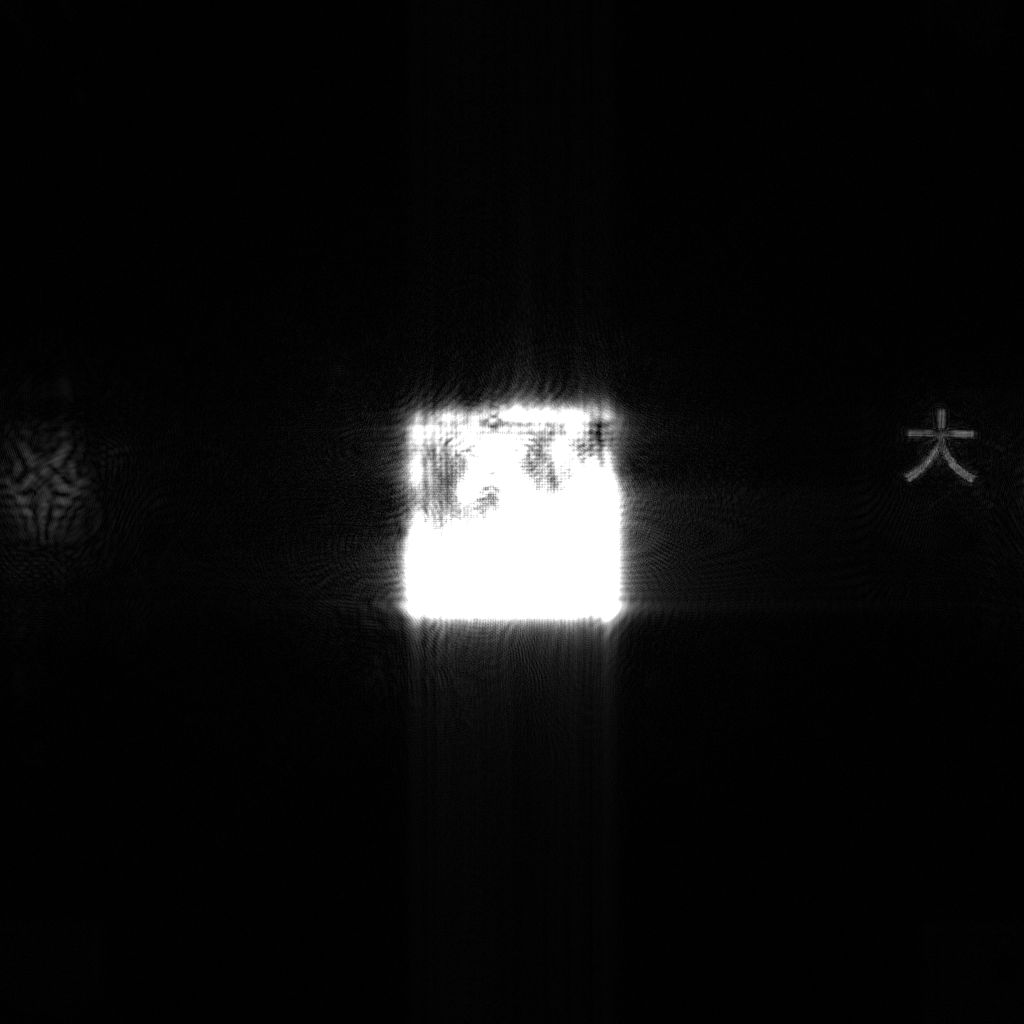
\includegraphics[width=.8\linewidth]{figs/3.png}
		\caption{再现图一}
	\end{figure}
	\begin{figure}[H]
		\centering
		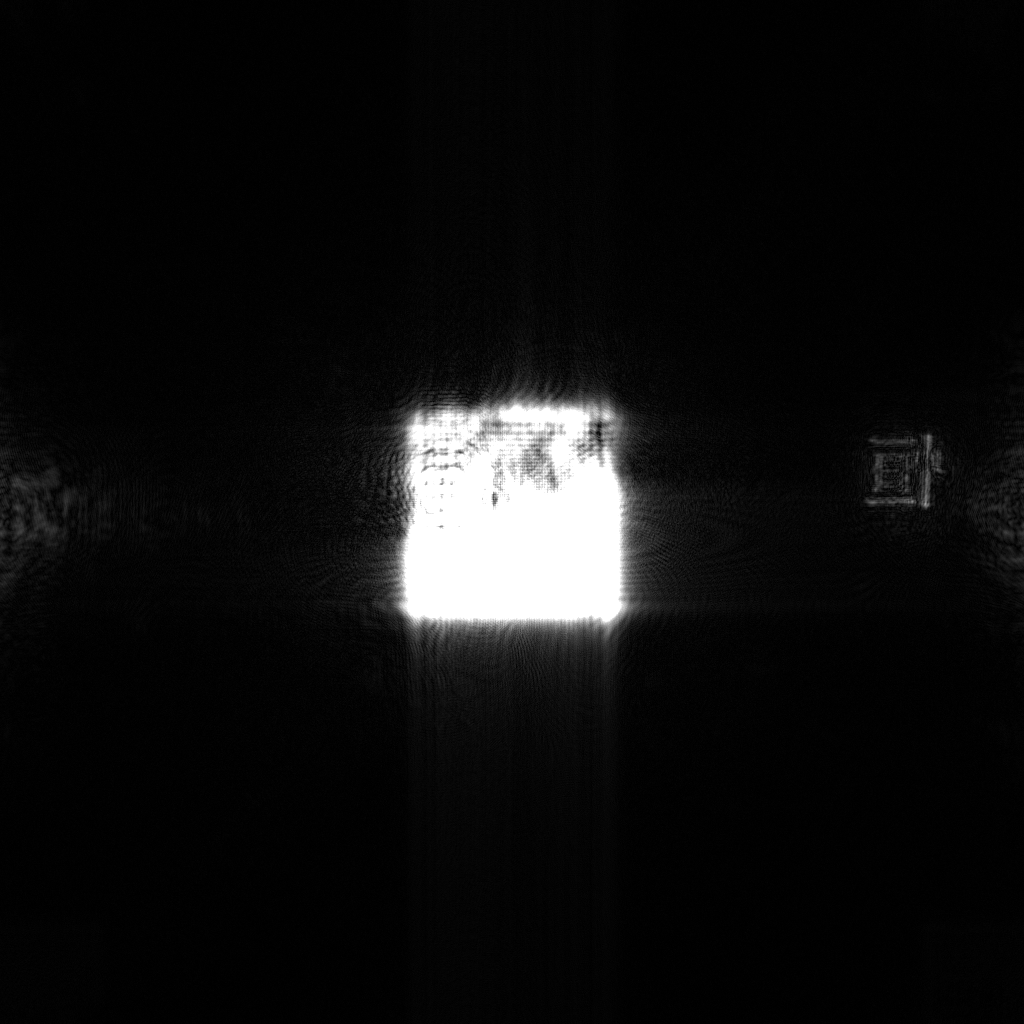
\includegraphics[width=.8\linewidth]{figs/4.png}
		\caption{再现图二}
	\end{figure}
	可以看到“大”、“恒”二字被清晰地再现了出来,实验中强度放大因子的大小设为3,如果设置的更大,再现像和周围之间的对比度会更高,效果应该会更好。
	\section{光学再现实验}
	根据光学再现的基本原理,搭建下图所示光路:
	\begin{figure}[H]
		\centering
		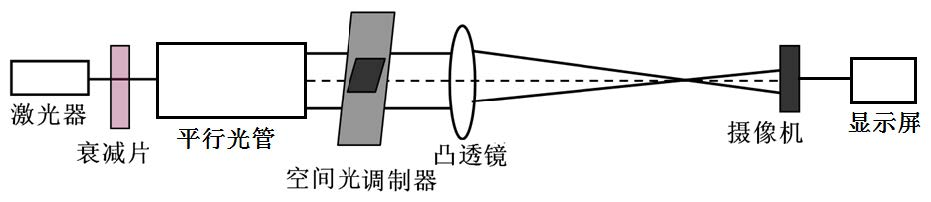
\includegraphics[width=\linewidth]{figs/光学再现.jpg}
		\caption{光学再现光路}
	\end{figure}
	将图\ref{fig1}和图\ref{fig2}的全息图加载到空间光调制器上,得到下面的再现图像:
	\begin{figure}[H]
		\centering
		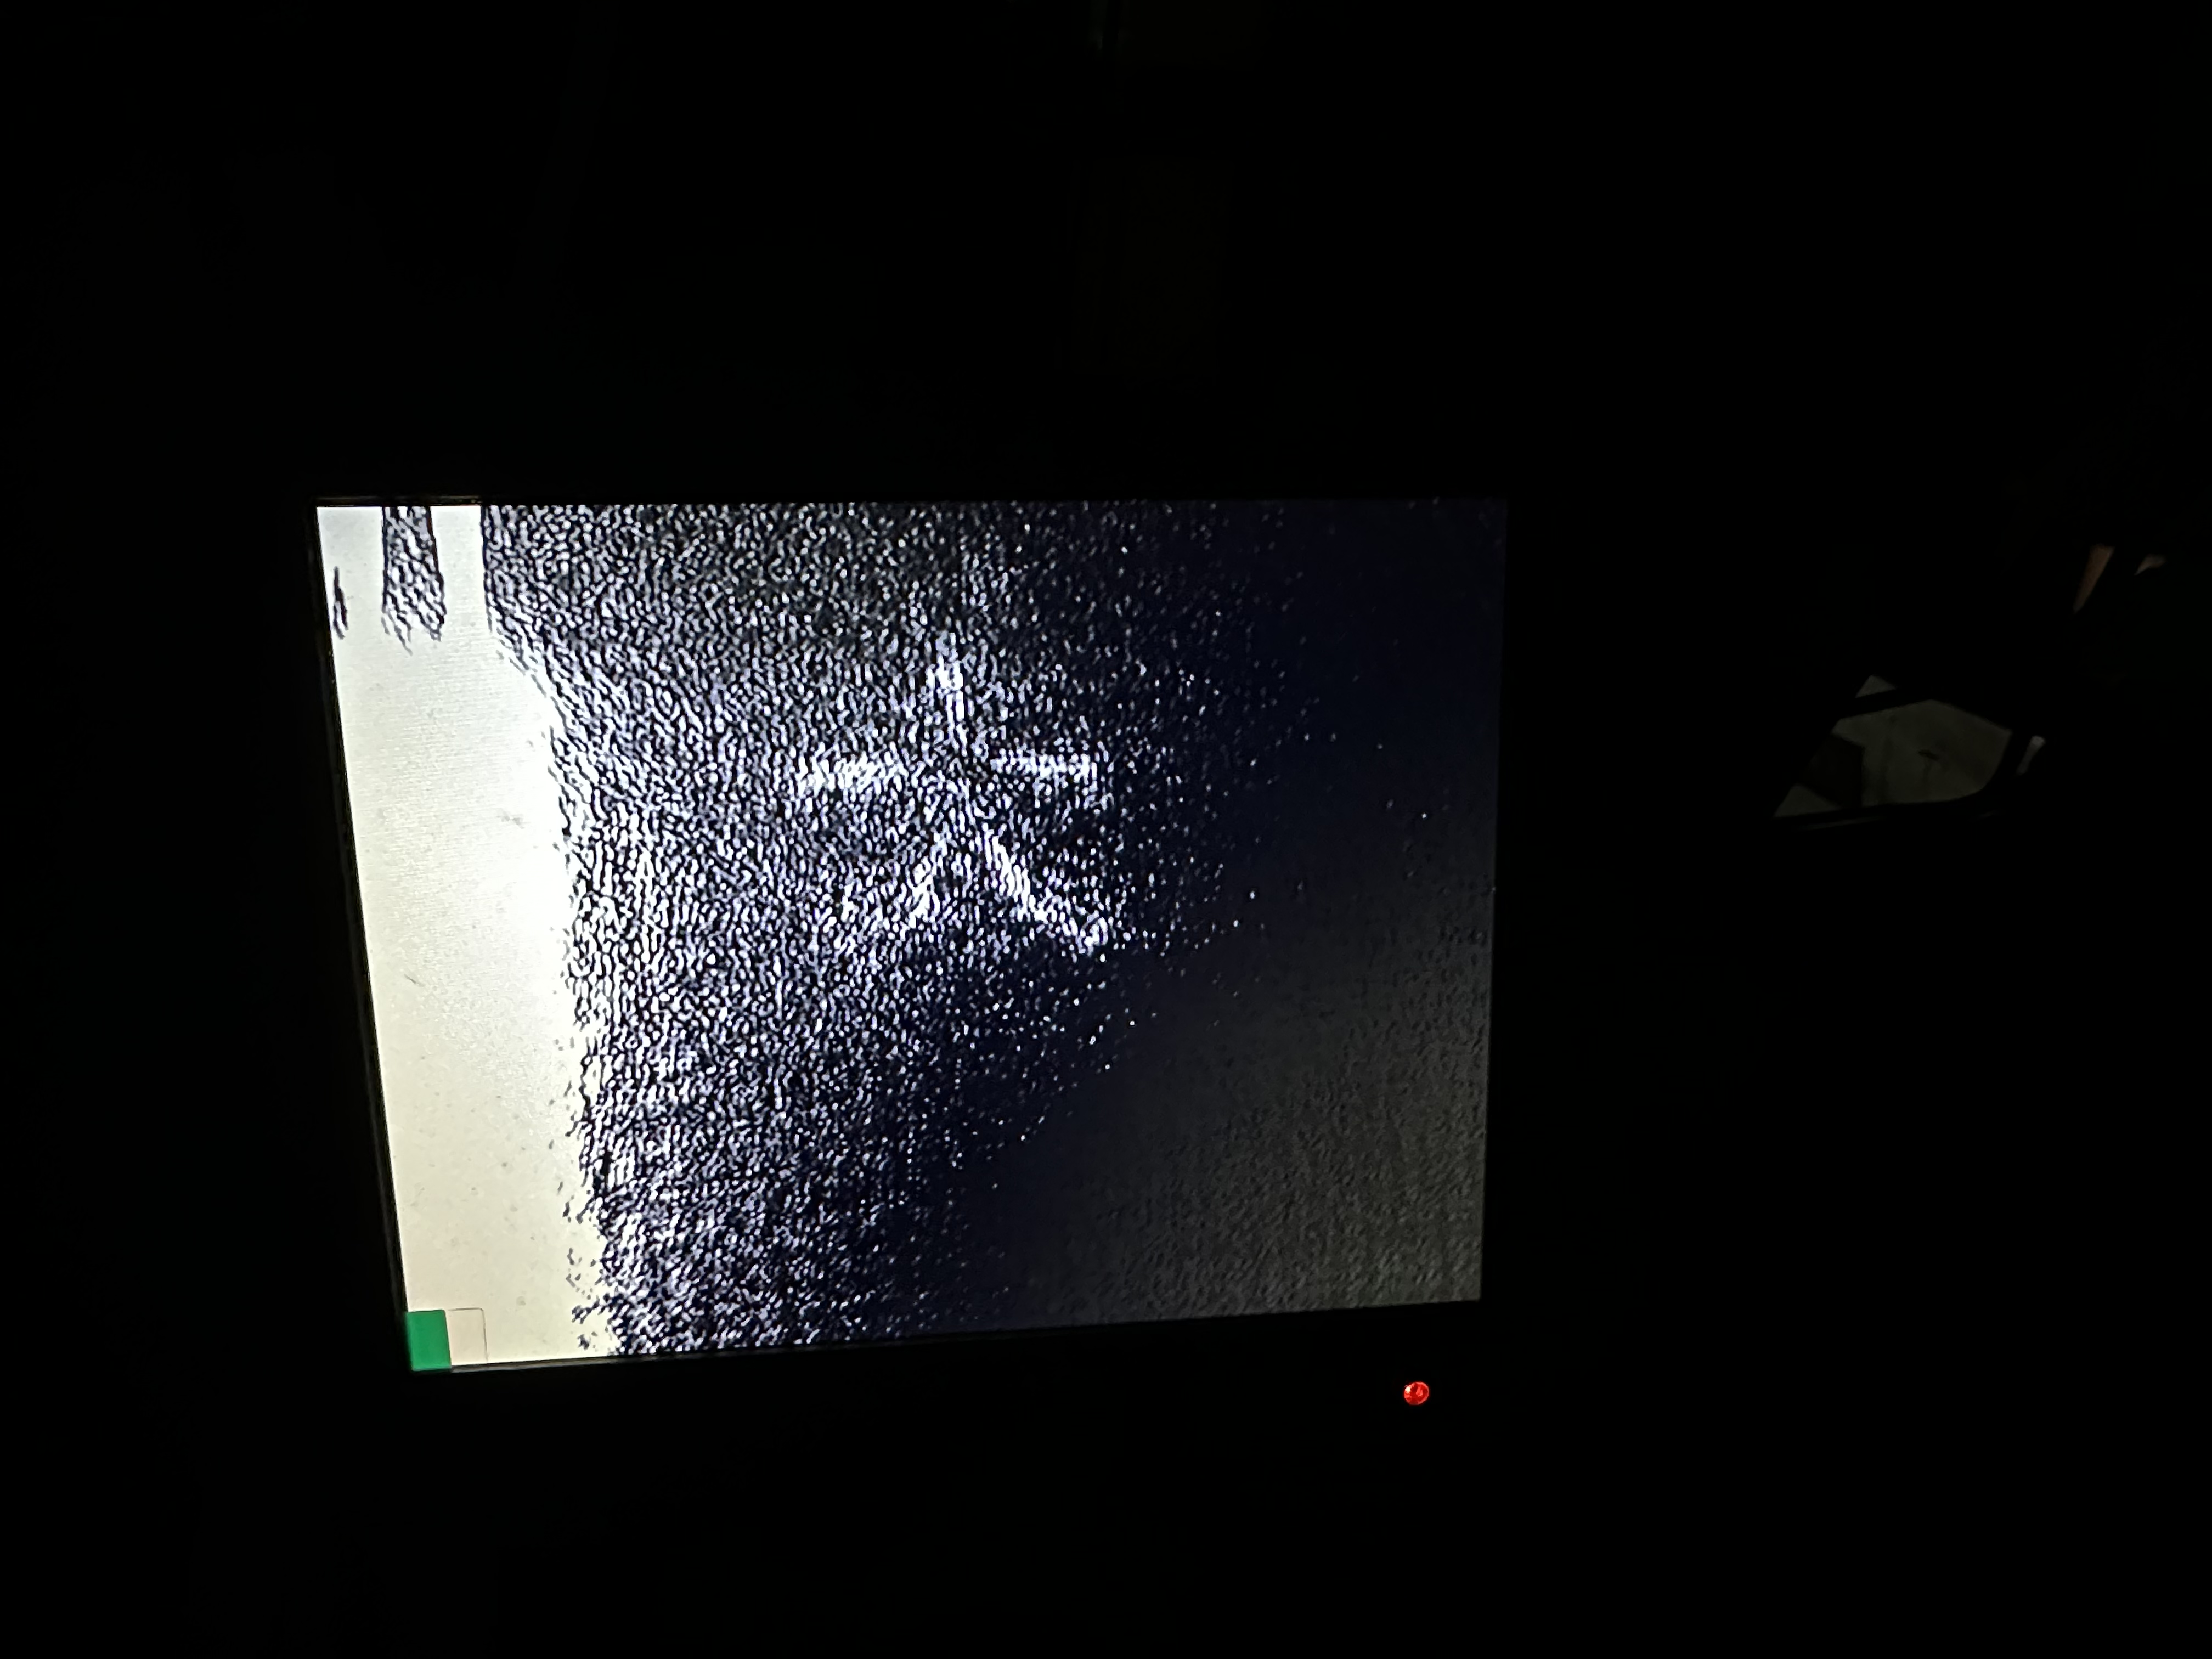
\includegraphics[width=.8\linewidth]{figs/5.jpg}
		\caption{光学再现图一}
	\end{figure}
	\begin{figure}[H]
		\centering
		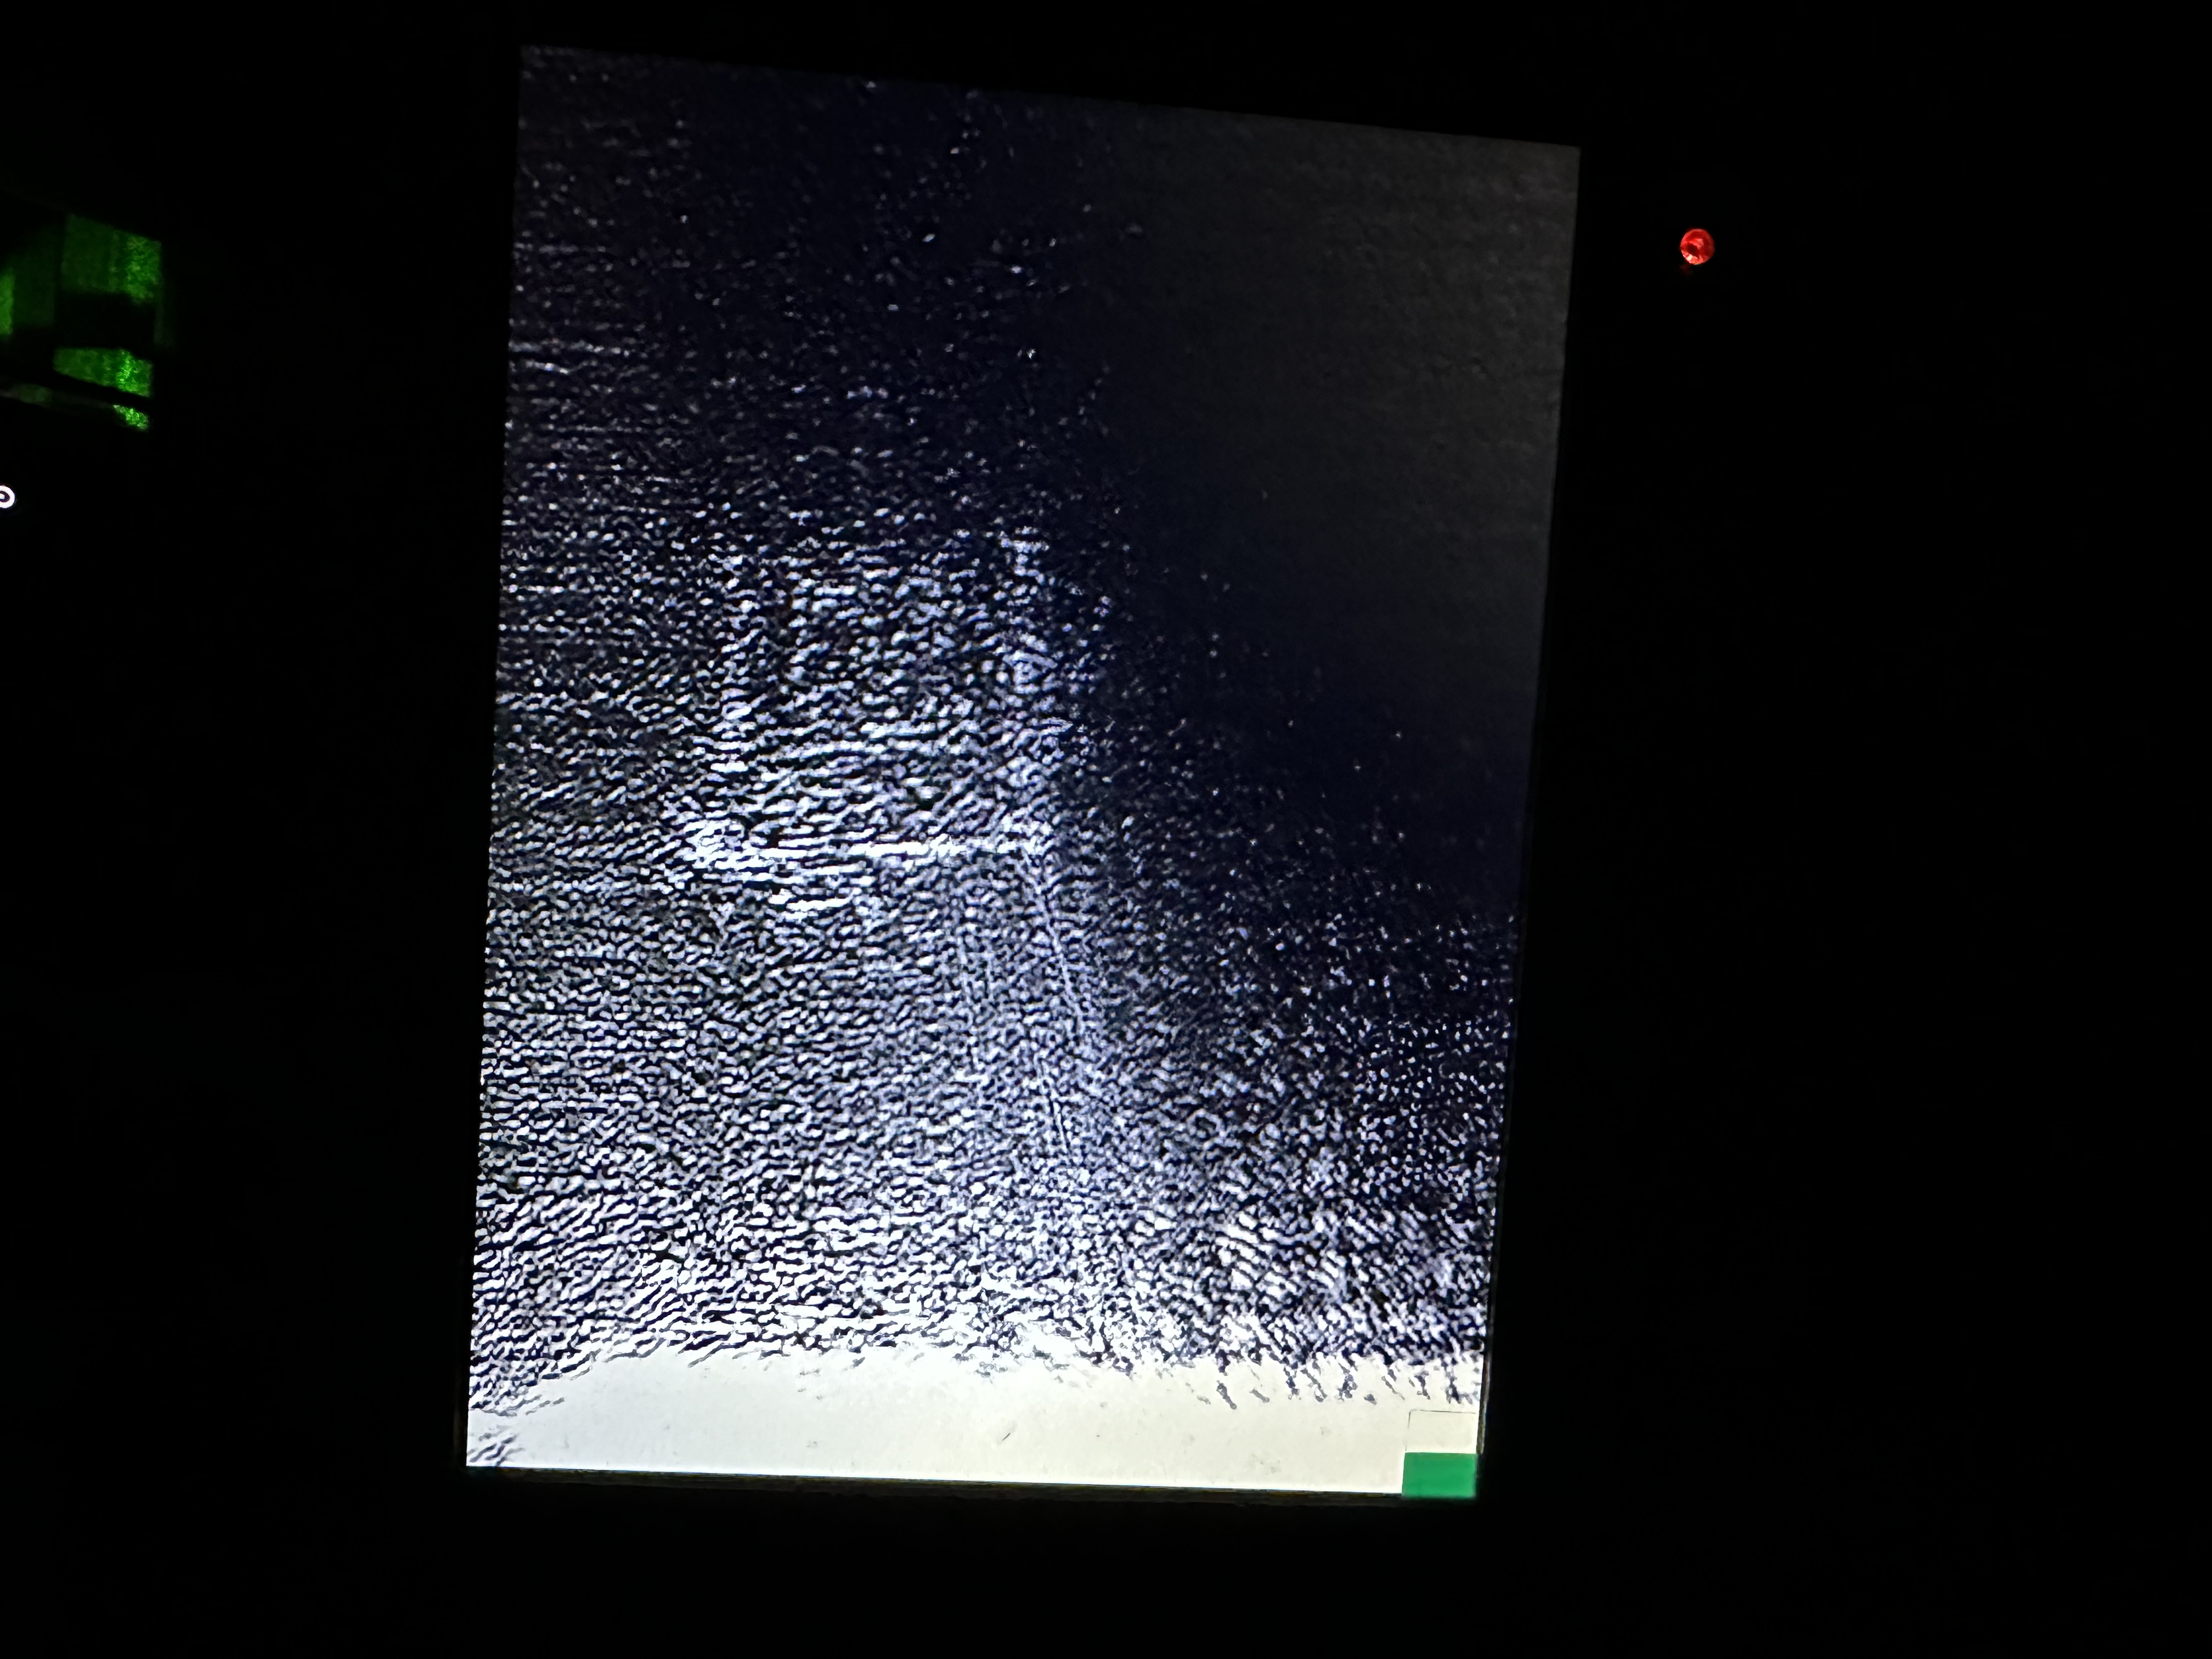
\includegraphics[width=.8\linewidth,=,angle=270]{figs/6.jpg}
		\caption{光学再现图二}
	\end{figure}
	\section{计算模拟全息}
	利用计算机软件模拟光波场,物体的图像为:
	\begin{figure}[H]
		\centering
		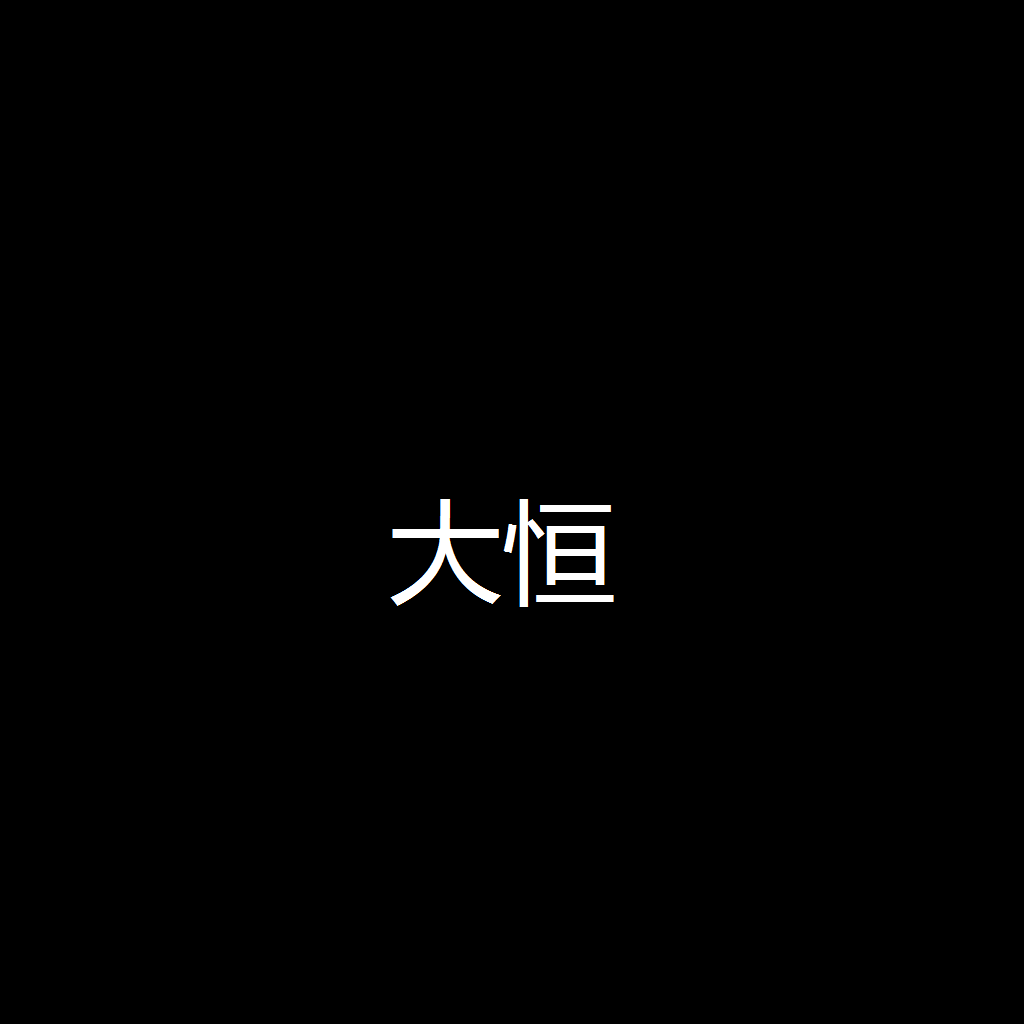
\includegraphics[width=.8\linewidth]{figs/7.png}
		\caption{物体图像“大恒”}
	\end{figure}
	直接计算出全息图:
	\begin{figure}[H]
		\centering
		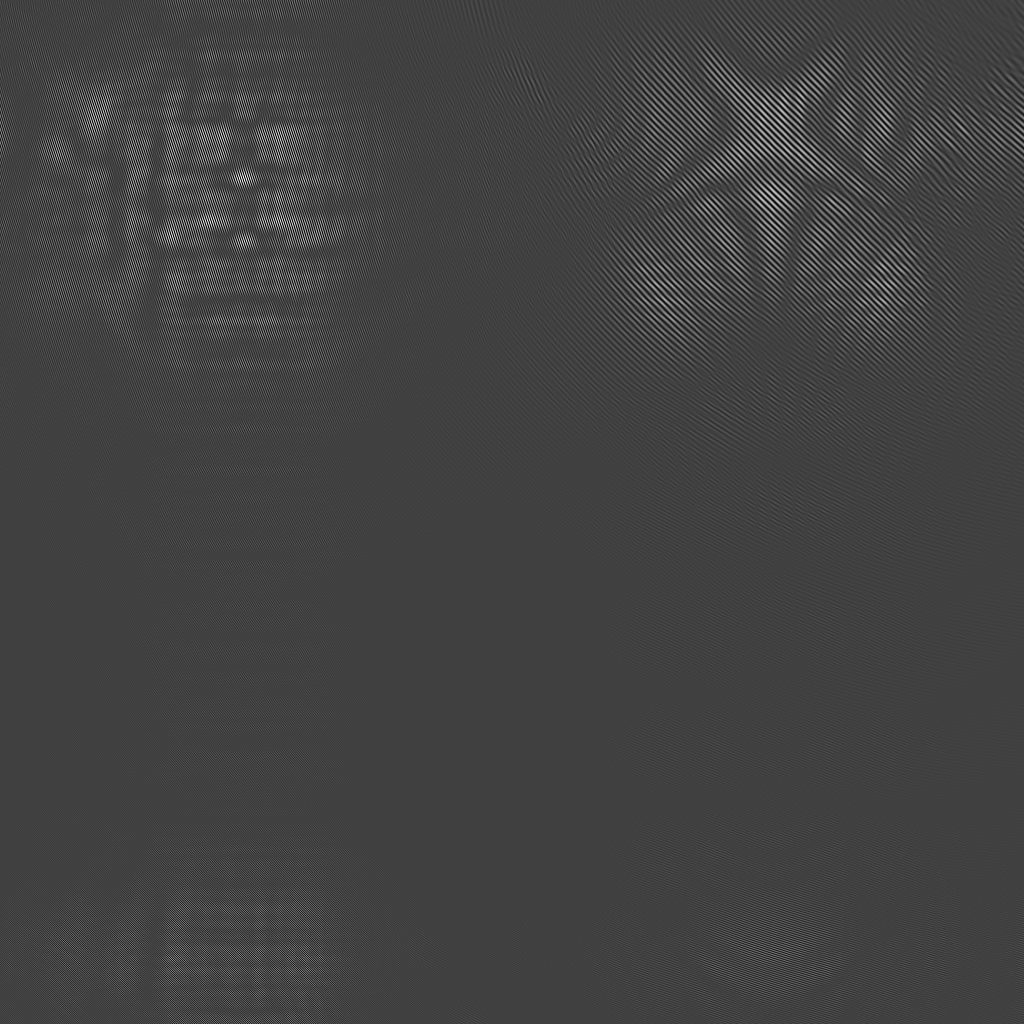
\includegraphics[width=.8\linewidth]{figs/8.png}
		\caption{计算模拟全息图——“大恒”}
	\end{figure}
	把上图和图\ref{fig1}和图\ref{fig2}的全息图对比,可以发现实验结果和理论计算预测结果吻合的非常好。再利用计算机计算重建模拟再现,得到:
	\begin{figure}[H]
		\centering
		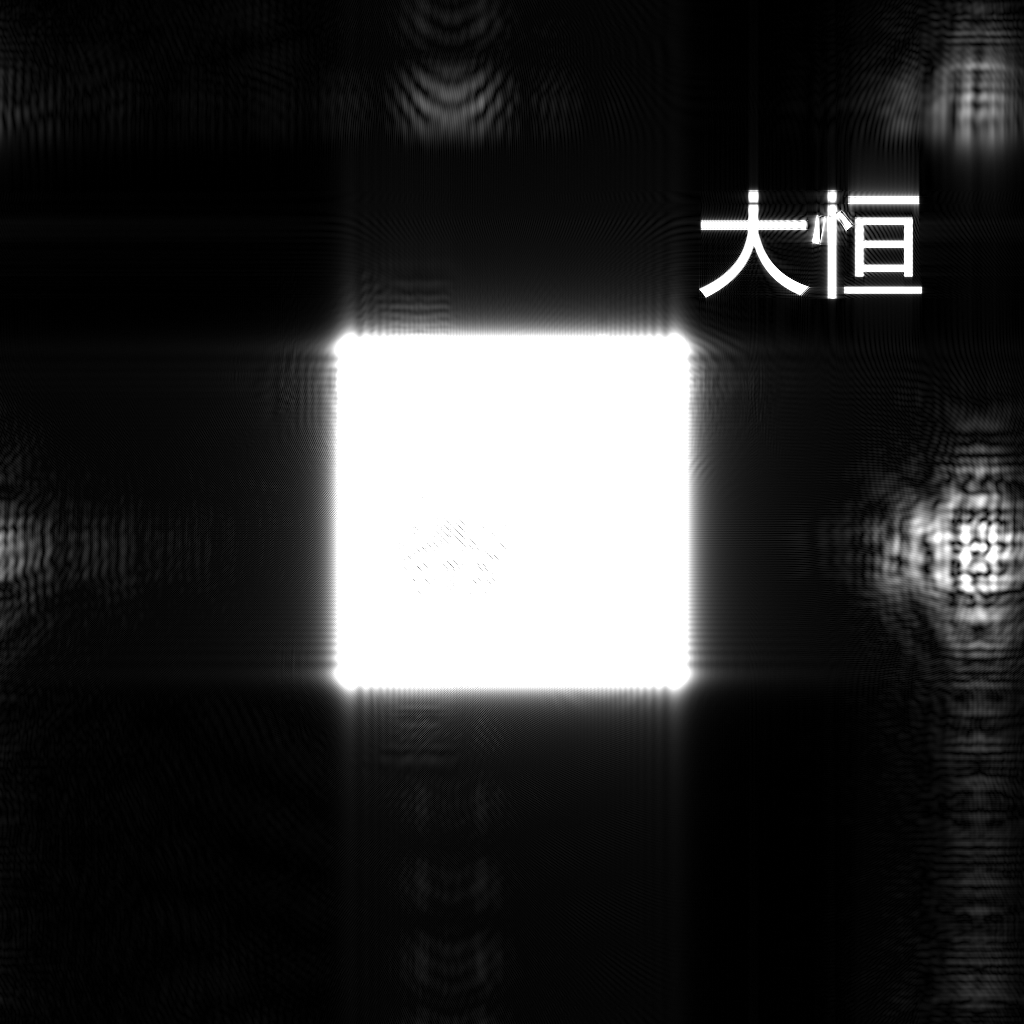
\includegraphics[width=.8\linewidth]{figs/9.png}
		\caption{计算模拟再现图——“大恒”}
	\end{figure}
	上图结果与光学再现和数字记录数字再现得到的结果非常相似,当然,由于实验存在很多干扰,所以再现图与周围环境的对比度以及分辨率不可能有数字模拟效果这么好。实验中是将“大”和“恒”分开进行实验的,这时因为实验中使用的平行光管的截面限制,导致照射到的物体大小存在限制。
	
	利用计算模拟得到的全息图,以及光学再现光路图,还可以得到计算模拟\mbox{-}光学再现图像为:
	\begin{figure}[H]
		\centering
		\includegraphics[width=.8\linewidth]{figs/10.jpg}
		\caption{计算模拟光学再现图}
	\end{figure}
	图中“恒”的对比度不高,不过“大”字仍旧清晰可见。
	\section{结\quad 论}
	本次实验利用CCD、空间光调制器和计算机软件搭建光路光学记录和再现了全息图,并于计算机重建得到的物体图像进行比对,在实验过程中加深了对光学数字全息以及采样定理的理解。实验上还利用计算机软件计算模拟了全息图,发现和实验上直接利用光路搭建得到的全息图吻合的非常好,利用计算得到的全息图进行光学再现也得到了不错的结果。本次实验还有不少可以扩展的地方,比如可以利用更加先进的计算机重建算法利用Matlab或者其它编程软件写一个重建算法,对图像进行一些预处理,得到的结果应该会更好。
	
	\bibliographystyle{unsrt}

	\begin{thebibliography}{99}  
		\bibitem{ref1}{J. W. Goodman, R. W. Lawrence; DIGITAL IMAGE FORMATION FROM ELECTRONICALLY DETECTED HOLOGRAMS. Appl. Phys. Lett. 1 August 1967; 11 (3): 77–79.}
		\bibitem{ref2}袁操今,翟宏琛,王晓雷等.采用短相干光数字全息术实现反射型微小物体的三维形貌测量[J].物理学报,2007(01):218-223.
		\bibitem{ref3}钟丽云,张以谟,吕晓旭等.数字全息图再现像的分析计算[J].中国激光,2004(05):570-574.
		\bibitem{ref4}王华英,王广俊,赵洁等.数字全息显微系统的成像分辨率分析[J].中国激光,2007(12):1670-1675.
		\bibitem{ref5}钱晓凡,董可平,张磊等.反射式数字全息显微术对细胞的研究[J].光子学报,2007(07):1318-1321.
		\bibitem{ref6}王大勇,崔华坤,王云新等.光学实验教学中引入数字全息实验的探讨[J].大学物理,2010,29(04):52-54+65.
		\bibitem{ref7}(美)约瑟夫·W.古德曼(Joseph W.Goodman) 著;陈家璧,秦克诚,曹其智 译. 傅里叶光学导论(第四版)[M]. 北京:科学出版社, 2020.
		\bibitem{ref8}张美玲,郜鹏,温凯等.同步相移数字全息综述(特邀)[J].光子学报,2021,50(07):9-31.
		\bibitem{ref9}陈浩. 离轴数字全息重建中消零级频谱滤波及衍射成像自聚焦研究[D].北京工业大学,2022.DOI:10.26935/d.cnki.gbjgu.2022.000434.
		\bibitem{ref10}吴晴晴,蒋世磊,张锦等.基于空间光调制器的动态全息再现技术研究[J].光学与光电技术,2023,21(02):65-71.DOI:10.19519/j.cnki.1672-3392.20230316.003.
		\bibitem{ref11}刘秋武.数字全息的计算机仿真[J].物理与工程,2010,20(04):45-48.
		\bibitem{ref12}郭苗苗. 计算全息生成和再现方法研究[D].西安电子科技大学,2014.
	\end{thebibliography}
\end{multicols}

\end{document}
